\documentclass{beamer}
\usepackage{beamerbasetoc}
\usepackage{beamerbaseoverlay}
\usepackage{enumitem}
\usepackage{bookmark}
\usepackage{graphicx} % Required for including images
\usepackage[absolute,overlay]{textpos} % Required for positioning elements absolutely
\usepackage{xcolor} % Required for defining colors
\usepackage{tikz}
\usepackage{pgfplots}
\pgfplotsset{compat=1.18}
\usepackage{xcolor}


% Define custom beamer color box for white background

\usecolortheme{default}
\setbeamercolor{hvidbox}{bg=white}

% Define custom color for KUrod
\definecolor{KUrod}{RGB}{144,26,30} % Change the RGB values to match the desired color

% Add page numbering to the footer
\setbeamertemplate{footline}{%
  \leavevmode%
  \hbox{%
  \begin{beamercolorbox}[wd=.9\paperwidth,ht=2.5ex,dp=1.125ex,leftskip=3ex,rightskip=3ex]{author in head/foot}%
    \usebeamerfont{author in head/foot}\hfill\insertframenumber{} / \inserttotalframenumber\hfill%
  \end{beamercolorbox}}%
  \vskip0pt%
}

\title{Sample Presentation}
\author{Your Name}
\date{\today}

\begin{document}

{
\setbeamertemplate{background}{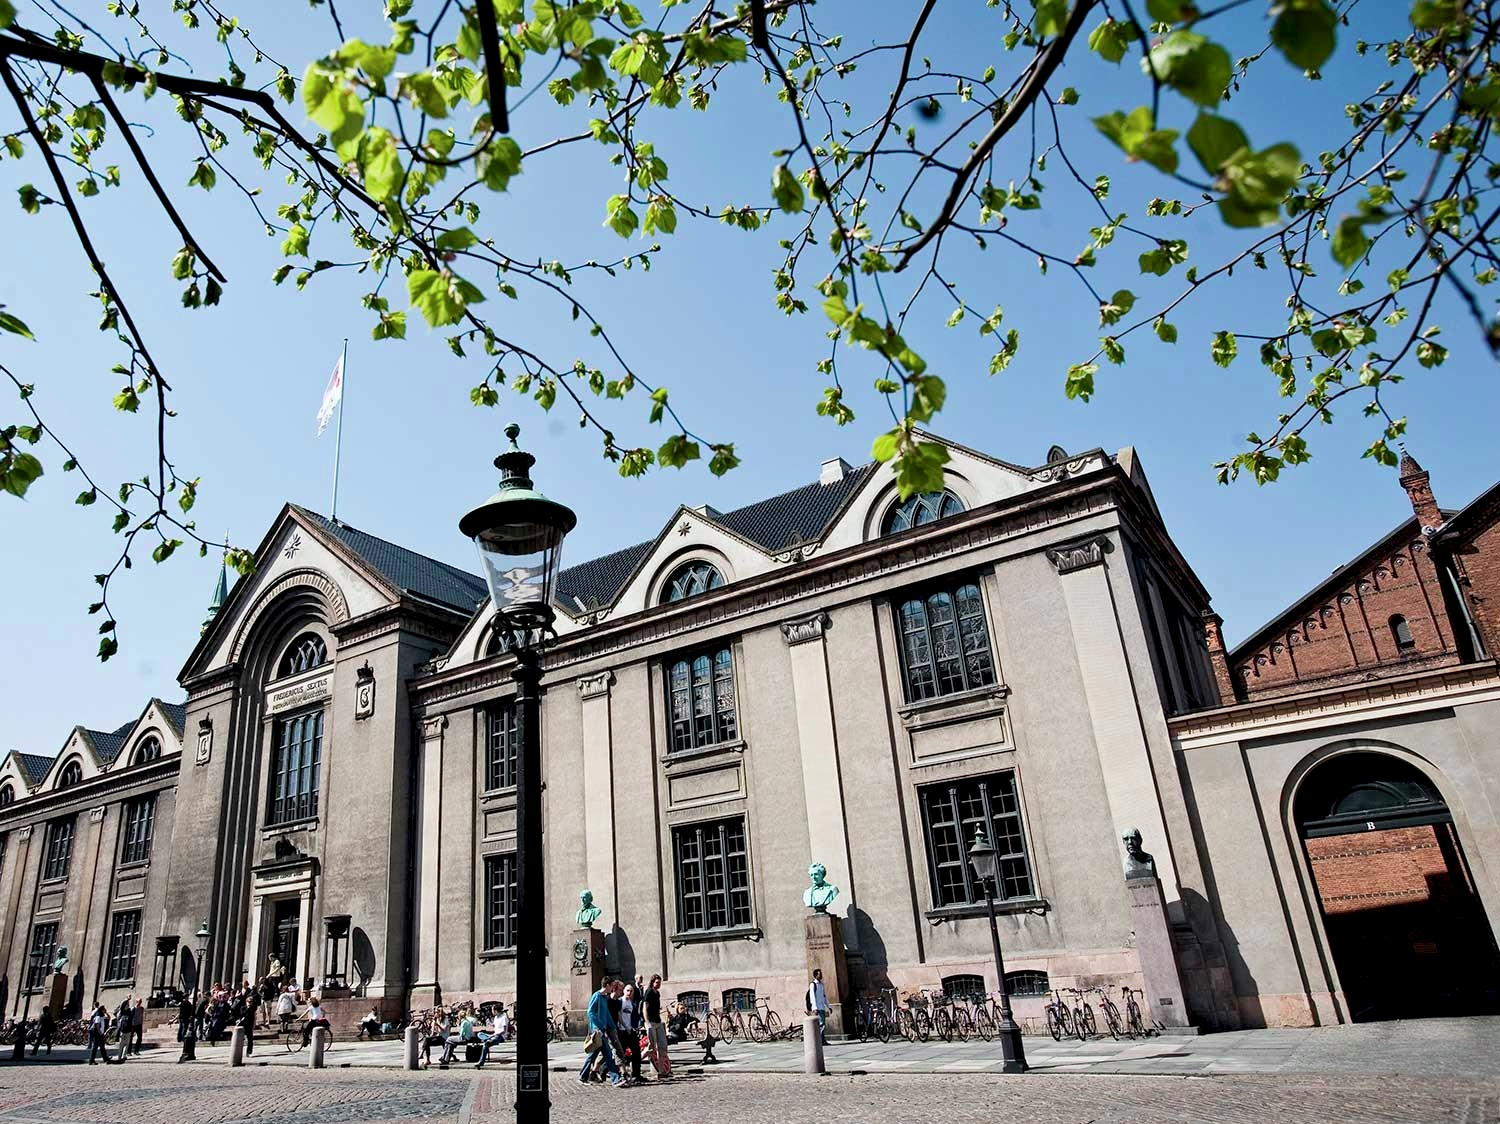
\includegraphics[width=\paperwidth,height=\paperheight]{/Users/nannaingemannohrt/Desktop/master_thesis/presentation/frontpage.jpg}}
\begin{frame}[plain] 
    \begin{textblock*}{\textwidth}(0.57\textwidth,0.1\textheight)
        \begin{beamercolorbox}[wd=7.8cm,ht=7.3cm,sep=0.5cm]{hvidbox}
            \fontsize{5}{10}\fontfamily{ptm}\selectfont \textls{UNIVERSITY OF COPENHAGEN}
            \noindent\textcolor{KUrod}{\rule{6.8cm}{0.4pt}}
        \end{beamercolorbox}
    \end{textblock*}
    \begin{textblock*}{\textwidth}(0.57\textwidth,0.2\textheight) 
        \begin{beamercolorbox}[wd=7.8cm,sep=0.5cm]{hvidbox}
                \Huge \textcolor{KUrod}{Master Thesis}
                \vspace{0.5cm}
                \par
                \Large Swaption Pricing Using the SABR Model
                \vspace{0.5cm}
                \par
                \normalsize Nanna Ingemann Ohrt
        \end{beamercolorbox}
    \end{textblock*}
    \begin{textblock}{1}(14.5,11.38)
        
\includegraphics[width=1cm]{/Users/nannaingemannohrt/Desktop/master_thesis/presentation/KU-logo.png}
    \end{textblock}
\end{frame}
}

\begin{frame}
    \frametitle{{\textcolor{KUrod}{Outline}}}
    \begin{itemize}[label=\textcolor{KUrod}{\textbullet}]
        \item Swaption As a Missing Link in Asset Allocation
        \item Mathematics of Pricing Swaptions
        \item One-Factor Short-Rate Model
        \item Constant Volatility
        \item The SABR Model
    \end{itemize}
\end{frame}
    

\section{Swaption As a Missing Link in Asset Allocation}
\begin{frame}
    \frametitle{\textcolor{KUrod}{Swaption As a Missing Link in Asset Allocation}}
    \begin{center}
        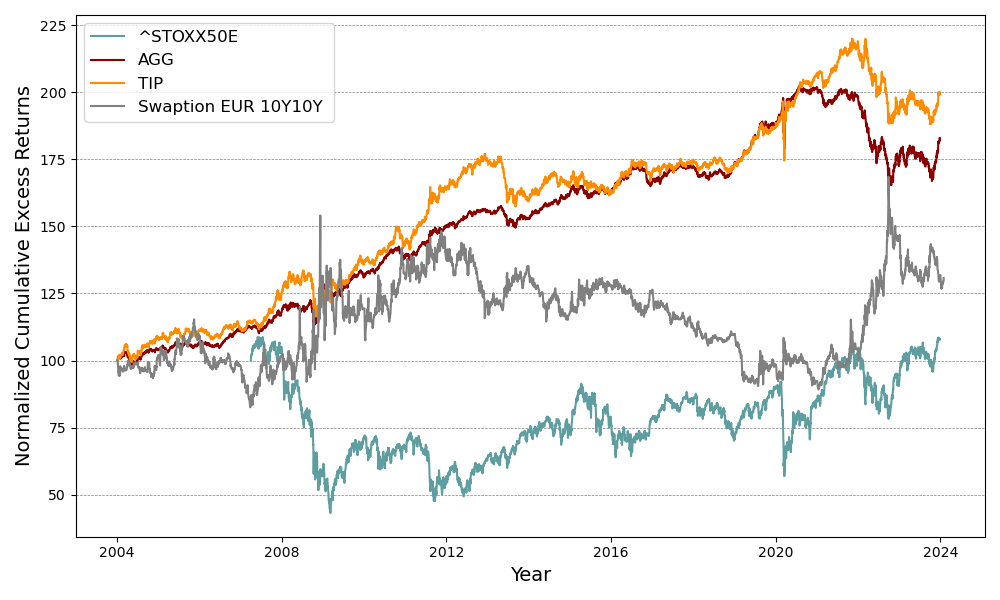
\includegraphics[width=0.8\textwidth]{/Users/nannaingemannohrt/Desktop/master_thesis/main/plots/2004_to_2024_plot.png}
    \end{center}
\end{frame}


\begin{frame}
    \frametitle{\textcolor{KUrod}{Swaption As a Missing Link in Asset Allocation}}
    \begin{columns}
        \column{0.5\textwidth}
        \begin{center}
            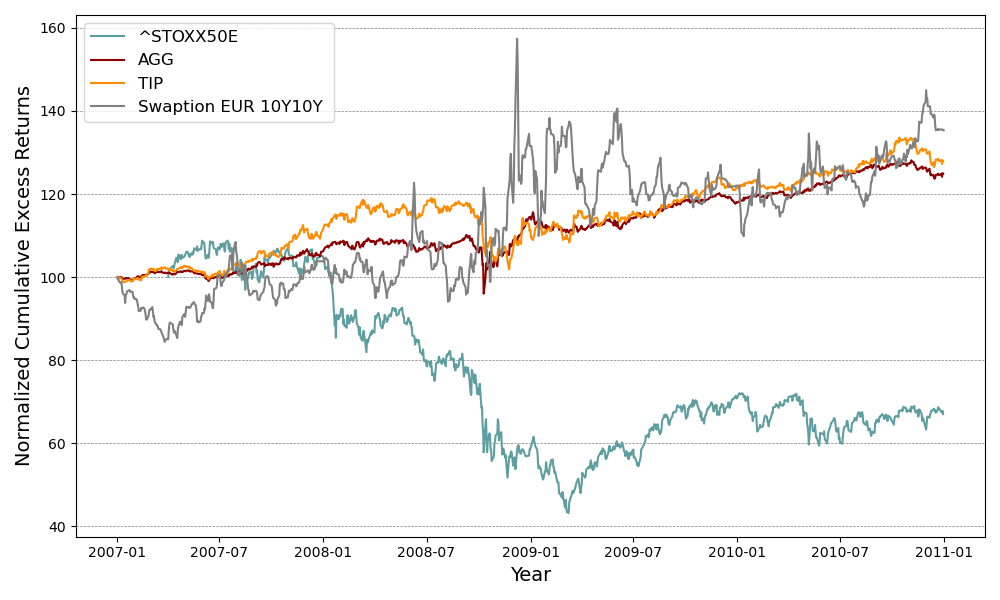
\includegraphics[width=\textwidth]{/Users/nannaingemannohrt/Desktop/master_thesis/main/plots/2007_to_2011.png}
            \caption{ Global Financial Crisis}
        \end{center}

        \column{0.5\textwidth}
        \begin{center}
            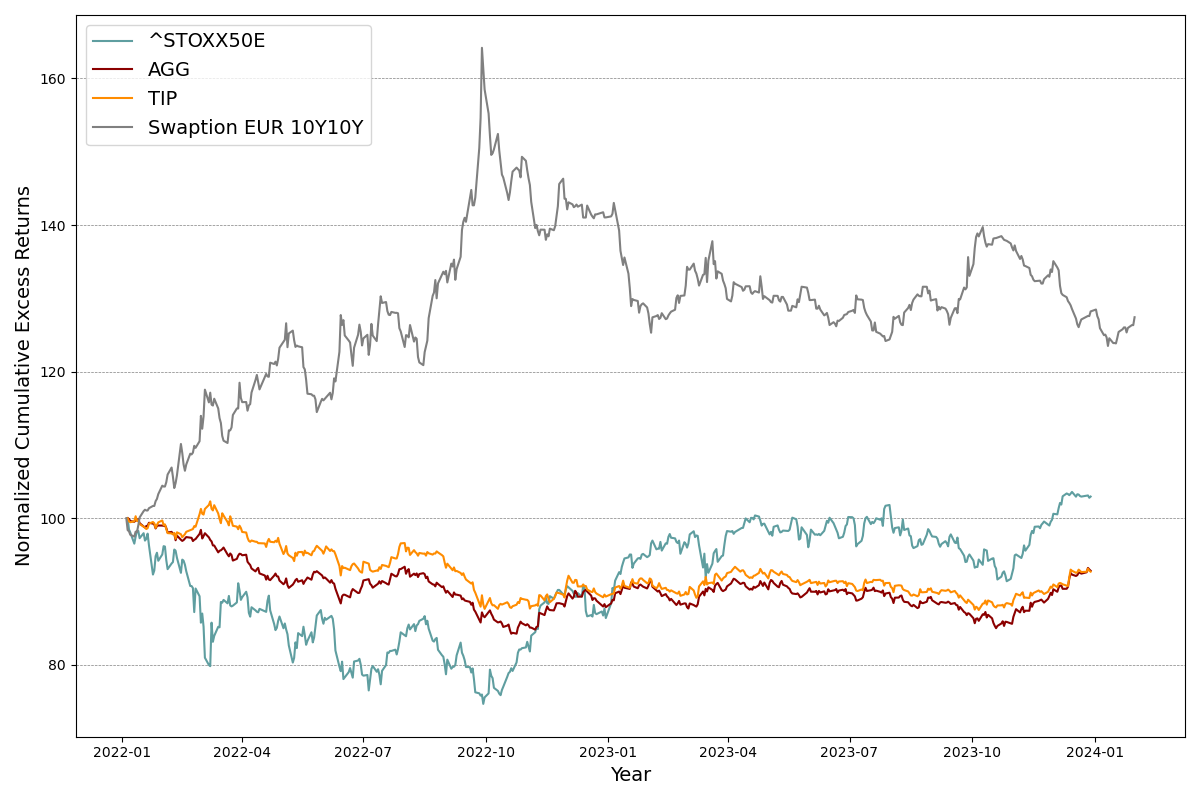
\includegraphics[width=\textwidth]{/Users/nannaingemannohrt/Desktop/master_thesis/main/plots/2022_to_2024.png}
            \captionof{}{ High inflation period}
        \end{center}
    \end{columns}
\end{frame}

\begin{frame}
    \frametitle{\textcolor{KUrod}{Mathematics of Pricing Swaptions}}
    A swaption is a financial derivative that can be described as an option to exchange a fixed rate bond for
    floating rate bonds for a predetermined principal. 
    There are two types of swaptions, payer swaptions and receiver swaptions.
    A payer swaption gives the holder the right to pay a fixed interest rate and receive a floating rate, 
    similar to a call option in the stock market. On the other hand, a receiver swaption allows the holder
    to pay a floating interest rate and receive a fixed rate, resembling a put option.
\end{frame} 

\begin{frame}
    \frametitle{\textcolor{KUrod}{Mathematics of Pricing Swaptions}}
        \begin{center}
            \begin{tikzpicture}[] 
                \draw[-latex] (5,0) -- (13,0) node[anchor=north] {Time};
                \draw (6,0.2) -- (6,-0.5) node[above] at (6.,0.3)  {t};
                \draw (11.5,-0.2) -- (11.5,0.5) node[below] at (11.5,-0.3) {T};
                \draw (11.75,1.5) rectangle (11.25,0.5);
                \draw (5.75,-1.5) rectangle (6.25,-0.5) node[below, pos=.01] {Principal Payment};
                \node at (11.5, 2.0) {Principal Repayment };
            \end{tikzpicture}\\[10pt] 
            Illustration 3.1: Cashflow for a zero coupon bond
        \end{center}
\end{frame}

\begin{frame}
    \frametitle{\textcolor{KUrod}{Mathematics of Pricing Swaptions}}
    \begin{center}
        \begin{tikzpicture} [scale=0.8]
            \draw[-Latex] (2,0) -- (10.5,0) node[anchor=north] {Time};
            \draw[thick, -Latex] (3,0) to [out=60,in=120] node[above] {$r_1$} (5,0);
            \draw[thick, -Latex] (5,0) to [out=60,in=120] node[above] {$r_2$} (7,0);
            \draw[thick, -Latex] (7,0) to [out=60,in=120] node[above] {$r_3$} (9,0);
            \draw[thick, -Latex] (3,0) to [out=-120,in=-60] node[below] {$l_1$} (5,0);
            \draw[thick, -Latex] (3,0) to [out=-120,in=-60] node[below] {$l_2$} (7,0);
            \draw[thick, -Latex] (3,0) to [out=-120,in=-60] node[below] {$l_3$} (9,0);
            \node at (2.7, -0.2) {0};
            \node at (4.7, -0.2) {1};
            \node at (6.7, -0.2) {2};
            \node at (8.7, -0.2) {3};
            \node at (0.1,0.5) {Forward rates:};
            \node at (0.1,-0.5) {Spot rates:};
        \end{tikzpicture}\\[10pt] 
        Illustration 3.3: Forward and spot rates
    \end{center}
\end{frame}

\begin{frame}
    \frametitle{\textcolor{KUrod}{Mathematics of Pricing Swaptions}}
        \begin{center}
            \begin{tikzpicture}[] 
                \draw[-latex] (5,0) -- (13,0) node[anchor=north] {Time};
                \draw (6,0.2) -- (6,-0.5) node[above] at (6.,0.3)  {t};
                \draw (11.5,-0.2) -- (11.5,0.5) node[below] at (11.5,-0.3) {T};
                \draw (11.75,1.5) rectangle (11.25,0.5) ;
                \draw (11.75,2) rectangle (11.25,1.5);
                \draw (5.75,-1.5) rectangle (6.25,-0.5) node[below, pos=.01] {Principal Payment};
                \draw[fill=black!15]  (10.5,0) rectangle (10.25,1);
                \draw[fill=black!15]  (8.5,0) rectangle (8.25,1);
                \draw[fill=black!15]  (9.5,0) rectangle (9.25,1);
                \draw[fill=black!15]  (7.5,0) rectangle (7.25,1);
                \node at (11.5, 2.5) {Principal Repayment};
                \node at (13.,1) {Principal Part};
                \node at (13.,1.75) {Interest Part};
                \node at (8.5, 1.5) {Periodic Fixed Interest Payments};
            \end{tikzpicture}\\[10pt] 
            Illustration 3.4: Cashflow for a fixed coupon bond
        \end{center}
\end{frame}


\begin{frame}
    \frametitle{\textcolor{KUrod}{Mathematics of Pricing Swaptions}}
    \begin{center}
        \begin{tikzpicture}[] 
            \draw[-latex] (5,0) -- (13,0) node[anchor=north] {Time};
            \draw (6,0.2) -- (6,-0.5) node[above] at (6.,0.3)  {t};
            \draw (12,-0.2) -- (12,0.5) node[below] at (12,-0.3) {T};
            \draw (12.25,1.5) rectangle (11.75,0.5) ;
            \draw (12.25,2) rectangle (11.75,1.5);
            \draw (5.75,-1.5) rectangle (6.25,-0.5) node[below, pos=.01] {Principal Payment};
            \draw[fill=black!15] (10.5,0) rectangle (10.25,1);
            \draw[fill=black!15]  (8.5,0) rectangle (8.25,1.5);
            \draw[fill=black!15]  (9.5,0) rectangle (9.25,1.2);
            \draw[fill=black!15] (7.5,0) rectangle (7.25,0.9);
            \node at (12, 2.6) {Principal Repayment};
            \node at (13.5,1) {Principal Part};
            \node at (13.5,1.75) {Interest Part};
            \node at (8.5, 1.8) {Periodic Floating Interest Payments};
        \end{tikzpicture}\\[10pt] 
        Illustration 3.5: Cashflow for a floating rate bond
    \end{center}
\end{frame}

\begin{frame}
    \frametitle{\textcolor{KUrod}{Mathematics of Pricing Swaptions}}
    \begin{center}
        \begin{tikzpicture}
            \tikzstyle{receiver} = [rectangle, fill=black!15, text centered, minimum height=3em]
            \tikzstyle{payer} = [rectangle,  fill=black!15, text centered, minimum height=3em]
            \node[receiver] (receiver) {Receiver};
            \node[payer, right of=receiver, node distance=8cm] (payer) {Payer};
            \draw[thick, <-] ([yshift=5pt]receiver.north) -- node[above] {Fixed rate} ([yshift=5pt]payer.north);
            \draw[thick, dashed, ->] ([yshift=-5pt]receiver.south) -- node[below] {Floating rate} ([yshift=-5pt]payer.south);
        \end{tikzpicture}\\[10pt] 
        Illustration 3.6: Cashflow for fixed and floating rate exchanges
    \end{center} 
\end{frame}

\begin{frame}
    \frametitle{\textcolor{KUrod}{Mathematics of Pricing Swaptions}}
    \begin{center}
        \begin{tikzpicture}
            \draw[thick] (0,0) -- (3.7,0);
            \draw[dashed](3.7,0) -- (5.7,0);
            \draw[thick] (5.7,0) -- (6.3,0);
            \draw[dashed](6.3,0) -- (8.2,0);
            \draw[thick] (8.2,0) -- (9.0,0);
            \draw[thick] (0.5,0.1) -- (0.5,-0.8) node at (0.3,-0.3) {t} ;
            \draw[thick] (2,0.1) -- (2,-0.8) node at (1.7,-0.3) {$T_S$} ;
            \draw[thick] (3.5,0.1) -- (3.5,-0.8) node at (3.05,-0.3) {$T_{S+1}$} ;
            \draw[thick] (6.0,0.1) -- (6.0,-0.8) node at (5.55,-0.3) {$T_{S+i}$} ;
            \draw[thick] (8.5,0.1) -- (8.5,-0.8) node at (8.15,-0.3) {$T_{E}$} ;
            \draw[decorate, decoration={zigzag, segment length=8pt, amplitude=4pt}] (3.5,0) -- node[above=15pt] {$\delta L(T_{S}, T_{S+1})$} (3.5,1.1);
            \draw[decorate, decoration={zigzag, segment length=8pt, amplitude=4pt}] (6,0) -- node[above=15pt] {$\delta L(T_{S+1}, T_{S+i})$} (6,1.1);
            \draw[decorate, decoration={zigzag, segment length=8pt, amplitude=4pt}] (8.5,0) -- node[above=15pt] {$\delta L(T_{E-1}, T_{E})$} (8.5,1.1);
            \node at (3.5,-1.) {$\delta$ K};
            \node at (6,-1.) {$\delta$ K};
            \node at (8.5,-1.) {$\delta$ K};
        \end{tikzpicture}\\[10pt] 
        Illustration 3.7: Cashflow for a payer swap 
    \end{center}
\end{frame}

\begin{frame}
    \frametitle{\textcolor{KUrod}{Mathematics of Pricing Swaptions}}
    Swaption pricing
\end{frame}
\begin{frame}
    \frametitle{\textcolor{KUrod}{One-Factor Short-Rate Model}}
    The Vasicek model 
    \begin{align}
        d r_t &= \kappa \Big[\theta - r(t)\Big] dt + \sigma d W(t) \label{vas_dyn1}\\
        r(0) &= r_0 \label{vas_dyn_r0}
    \end{align}
    \begin{center}
        \begin{minipage}{0.5\textwidth}
            \centering
            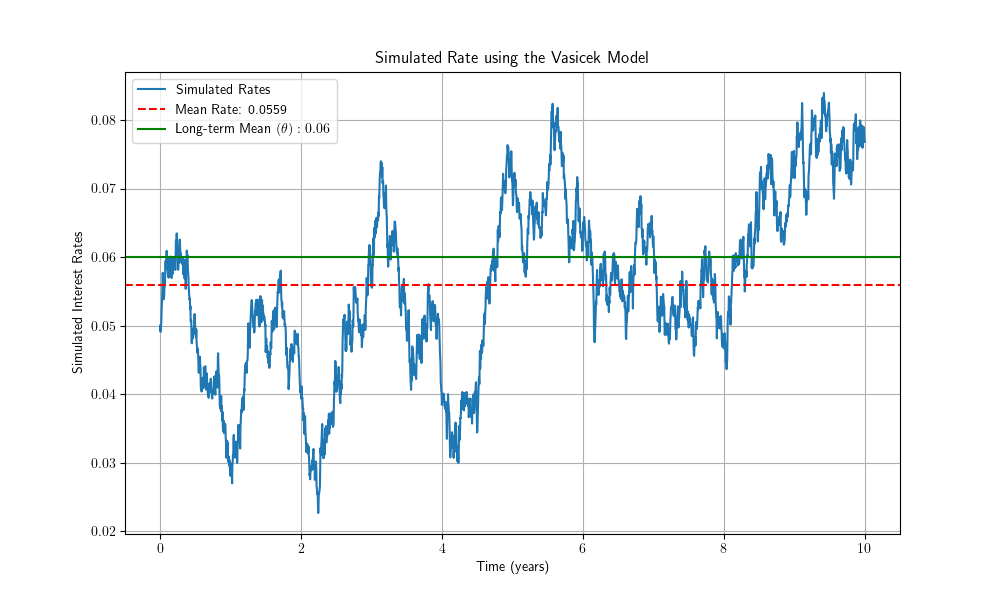
\includegraphics[width=\textwidth]{/Users/nannaingemannohrt/Desktop/master_thesis/main/plots/VasicekModelPlot.png}
            \captionof{}{}
        \end{minipage}\hfill
        \begin{minipage}{0.5\textwidth}
            \centering
            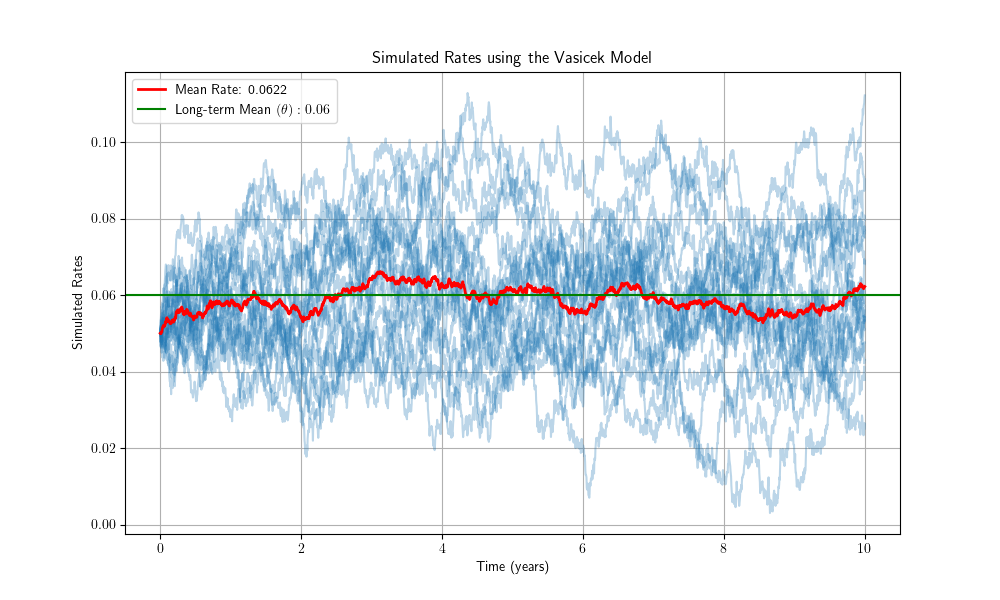
\includegraphics[width=\textwidth]{/Users/nannaingemannohrt/Desktop/master_thesis/main/plots/VasicekModelPlotSIM.png}
            \captionof{}{}
        \end{minipage}
    \end{center}
\end{frame}

\begin{frame}
    \frametitle{\textcolor{KUrod}{Constant Volatility}}
    \begin{columns}
        \column{0.5\textwidth}
        \begin{figure}
            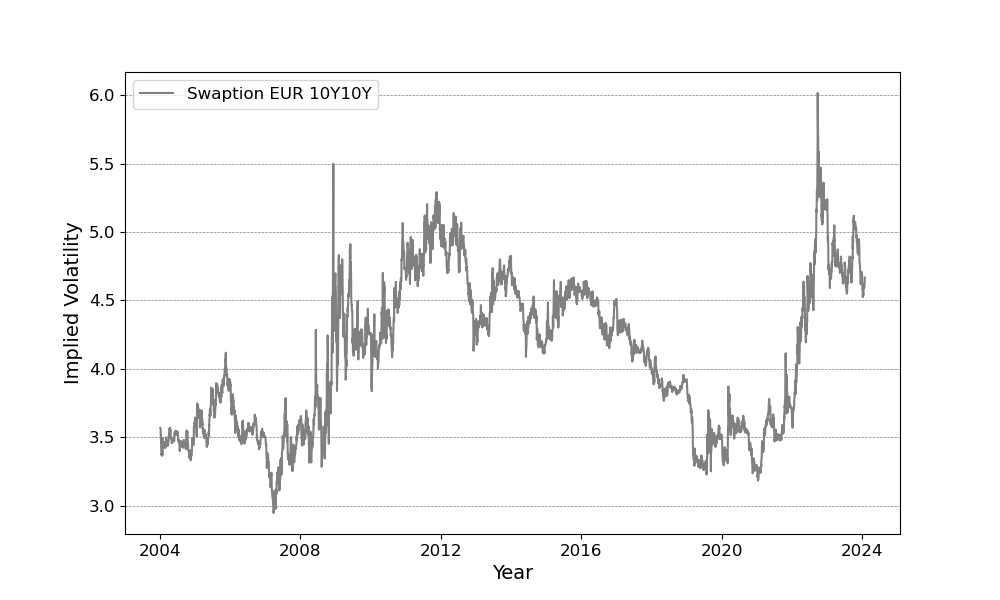
\includegraphics[width=\linewidth]{/Users/nannaingemannohrt/Desktop/master_thesis/main/plots/10Y10Yswaption.png}
        \end{figure}
        
        \begin{figure}
            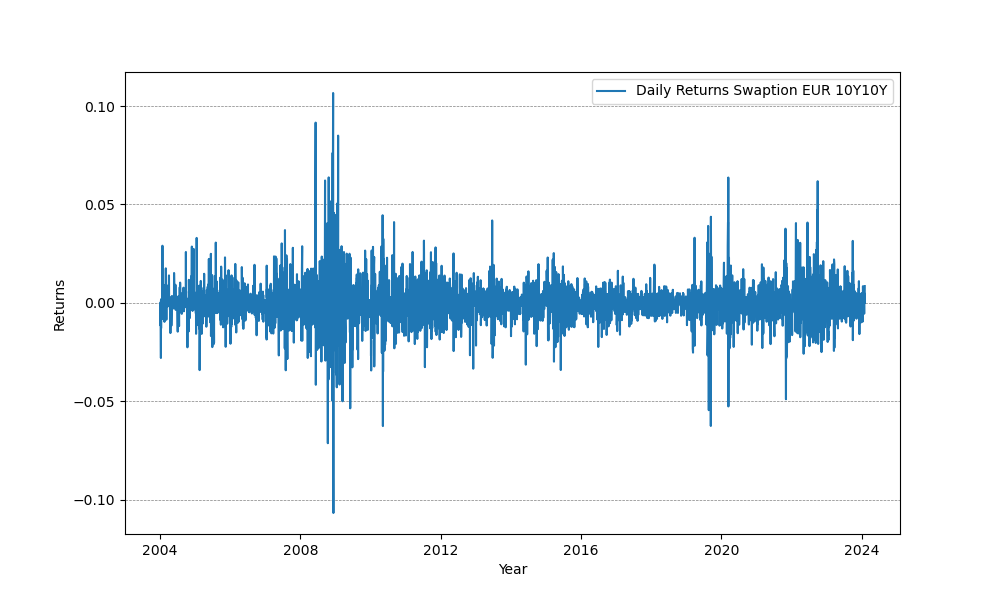
\includegraphics[width=\linewidth]{/Users/nannaingemannohrt/Desktop/master_thesis/main/plots/10Y10Yswaptionreturn.png}
        \end{figure}

        \column{0.5\textwidth}
        \begin{figure}
            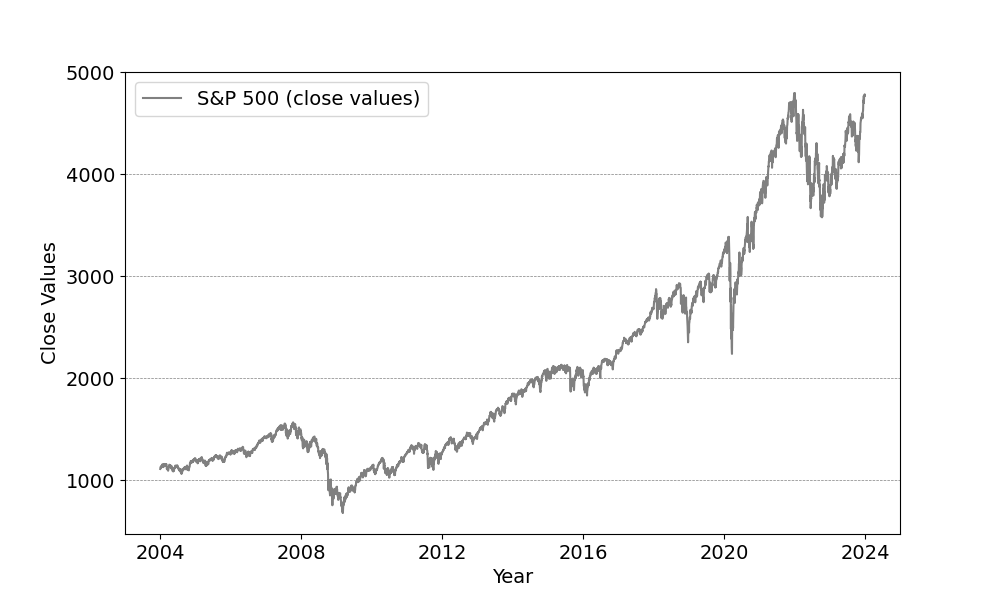
\includegraphics[width=\linewidth]{/Users/nannaingemannohrt/Desktop/master_thesis/main/plots/sp500.png}
        \end{figure}
        
        \begin{figure}
            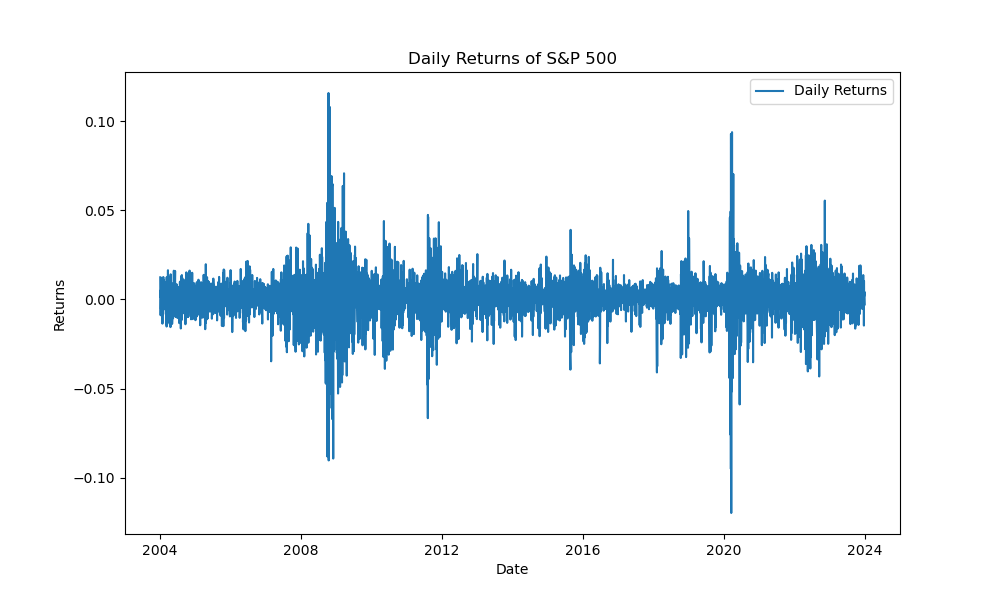
\includegraphics[width=\linewidth]{/Users/nannaingemannohrt/Desktop/master_thesis/main/plots/sp500return.png}
        \end{figure}
    \end{columns}

\end{frame}

\begin{frame}
    \frametitle{\textcolor{KUrod}{The SABR Model}}
\end{frame}


\end{document}
